\section{Background}
\label{sec:background}

In this section we cover the background of Namecoin. We begin by looking at the history of the cryptocurrency and then explain why a block chain can be used for our definition of a namespace. We then proceed to discuss the technical design of Namecoin and the mechanisms used in the design. We conclude this section with discussion about the applications of Namecoin.

\subsection{History}

Namecoin is an alternative cryptocurrency modeled after Bitcoin\cite{nakamoto2008bitcoin}. Furthermore, it is the first altcoin in the sense that it was the first to create its own block chain, separate from Bitcoin's.  Namecoin shares many similarities with Bitcoin, including the same method for proof of work, the same coin cap, the same block creation time, and all of the same transaction operations (with a few additions). Namecoin was inspired after discussions about a BitDNS\cite{bitdns} protocol using a block chain to manage a domain name lookup service. The idea behind this was that a central authority managing domain names, such as ICANN, requires too much trust in a single entity. Having a decentralized name system described by BitDNS provides resistance against a single point of failure. The first Namecoin block was mined in April 2011, and as of the writing of this paper, over 215,000 total blocks have been mined in the Namecoin system. Because of its similarities with Bitcoin, Namecoin was able to be merge-mined and has been merge-mined with Bitcoin since October 8, 2011. 

\subsection{How The block chain Works}

The block chain is a key feature to any Bitcoin based cryptocurrency. The block chain is a globally visible decentralized ledger. The ledger is maintained by all of the miners in the system. If a user wishes to move some of their coins, they create a transaction that describes which addresses the coins are coming from and which addresses the coins are going to, and then broadcasts the transaction to miners. If the next miner to mine a block has seen this transaction, they will try to include the transaction in their block.
    The key insight to use a block chain as a namespace is that the block chain can store more than just coin transactions. A block chain makes a good decentralized namespace because everyone who uses the system will have the same block chain (and hence the namespace data) stored on their machine. The reason why everyone has the same block chain returns us to Bitcoin and the concept of proof-of-work. Essentially everyone agrees that the block chain that is the longest (that has the most proof-of-work) is correct. This proof-of-work is what makes it computationally infeasible for an adversary to trick someone into believing a false block chain. 

{\bf block chain security.}
The value and stability of a cryptocurency are directly related to the amount of proof-of-work involved in the calculations of the blocks because this work is what keeps the data distributed and secure. For both Bitcoin and Namecoin, the proof-of-work is shown by calculating the hash of a new block and a random nonce over and over until the calculated hash has a certain number of leading zeros. The number of leading zeros required by the hash is referred to as the difficulty threshold. Namecoin enjoys a very high difficulty threshold for the proof of work. Namecoin is able to do this because it is similar to Bitcoin and supports merge mining with Bitcoin. This allows miners who are mining Bitcoin to also mine Namecoin at the same time with no extra work for the miner. Essentially, this is because the miner is using their computational power to solve a cryptographic puzzle that satisfies the proof-of-work for both block chains at the same time. This is advantageous for the miners because they are rewarded with coins from both systems, and helps Namecoin because it gives the Namecoin network a vastly increased amount of hash power over what it would have if it did not support merged mining. The high hash power and difficulty of the cryptographic challenge on the Namecoin network increases the stability of the system, providing resilience to a 51\% attack and other threatening behaviours from malicious miners.

\subsection{Technical Details of Names}

In this section and the next, we make an effort to differentiate between the technical details of the Namecoin name/value implementation and the specific mechanism design choices in Namecoin. The feature that separates Namecoin from Bitcoin is that Namecoin is a namespace, and can be used to register name/value pairs that can be stored in the block chain and traded amongst individuals. This registration is done using the three script operations exclusive to Namecoin: NAME\_NEW, NAME\_FIRSTUPDATE, and NAME\_UPDATE. In order to understand the registration process, we think it is helpful to walk through the registration process of a name, roughly following Figure \ref{fig:registration}. 

To start, the user will need to select a coin to be crafted into a token (or special coin) that represents a name and whose value can be changed by whoever possess the token. The next step to register a name is to make a transaction that uses the NAME\_NEW script operation in a transaction sending the token from one of their addresses to another. Using NAME\_NEW, a user can indicate an interest in a new name for a name/value pair by posting a hash commitment of the desired name in the scriptPubKey of the transaction. The NAME\_NEW operation acts as a signal in the block chain for name parsers to indicate that the next part of the scriptPubKey will be the hash commitment of a name. The protocol then places an OP\_2DROP on the stack to remove all of the name information put on the stack with the NAME\_NEW operation so that the rest of the locking portion of the scriptPubKey can function just as it does in Bitcoin. 

\begin{figure*}
  \centering
  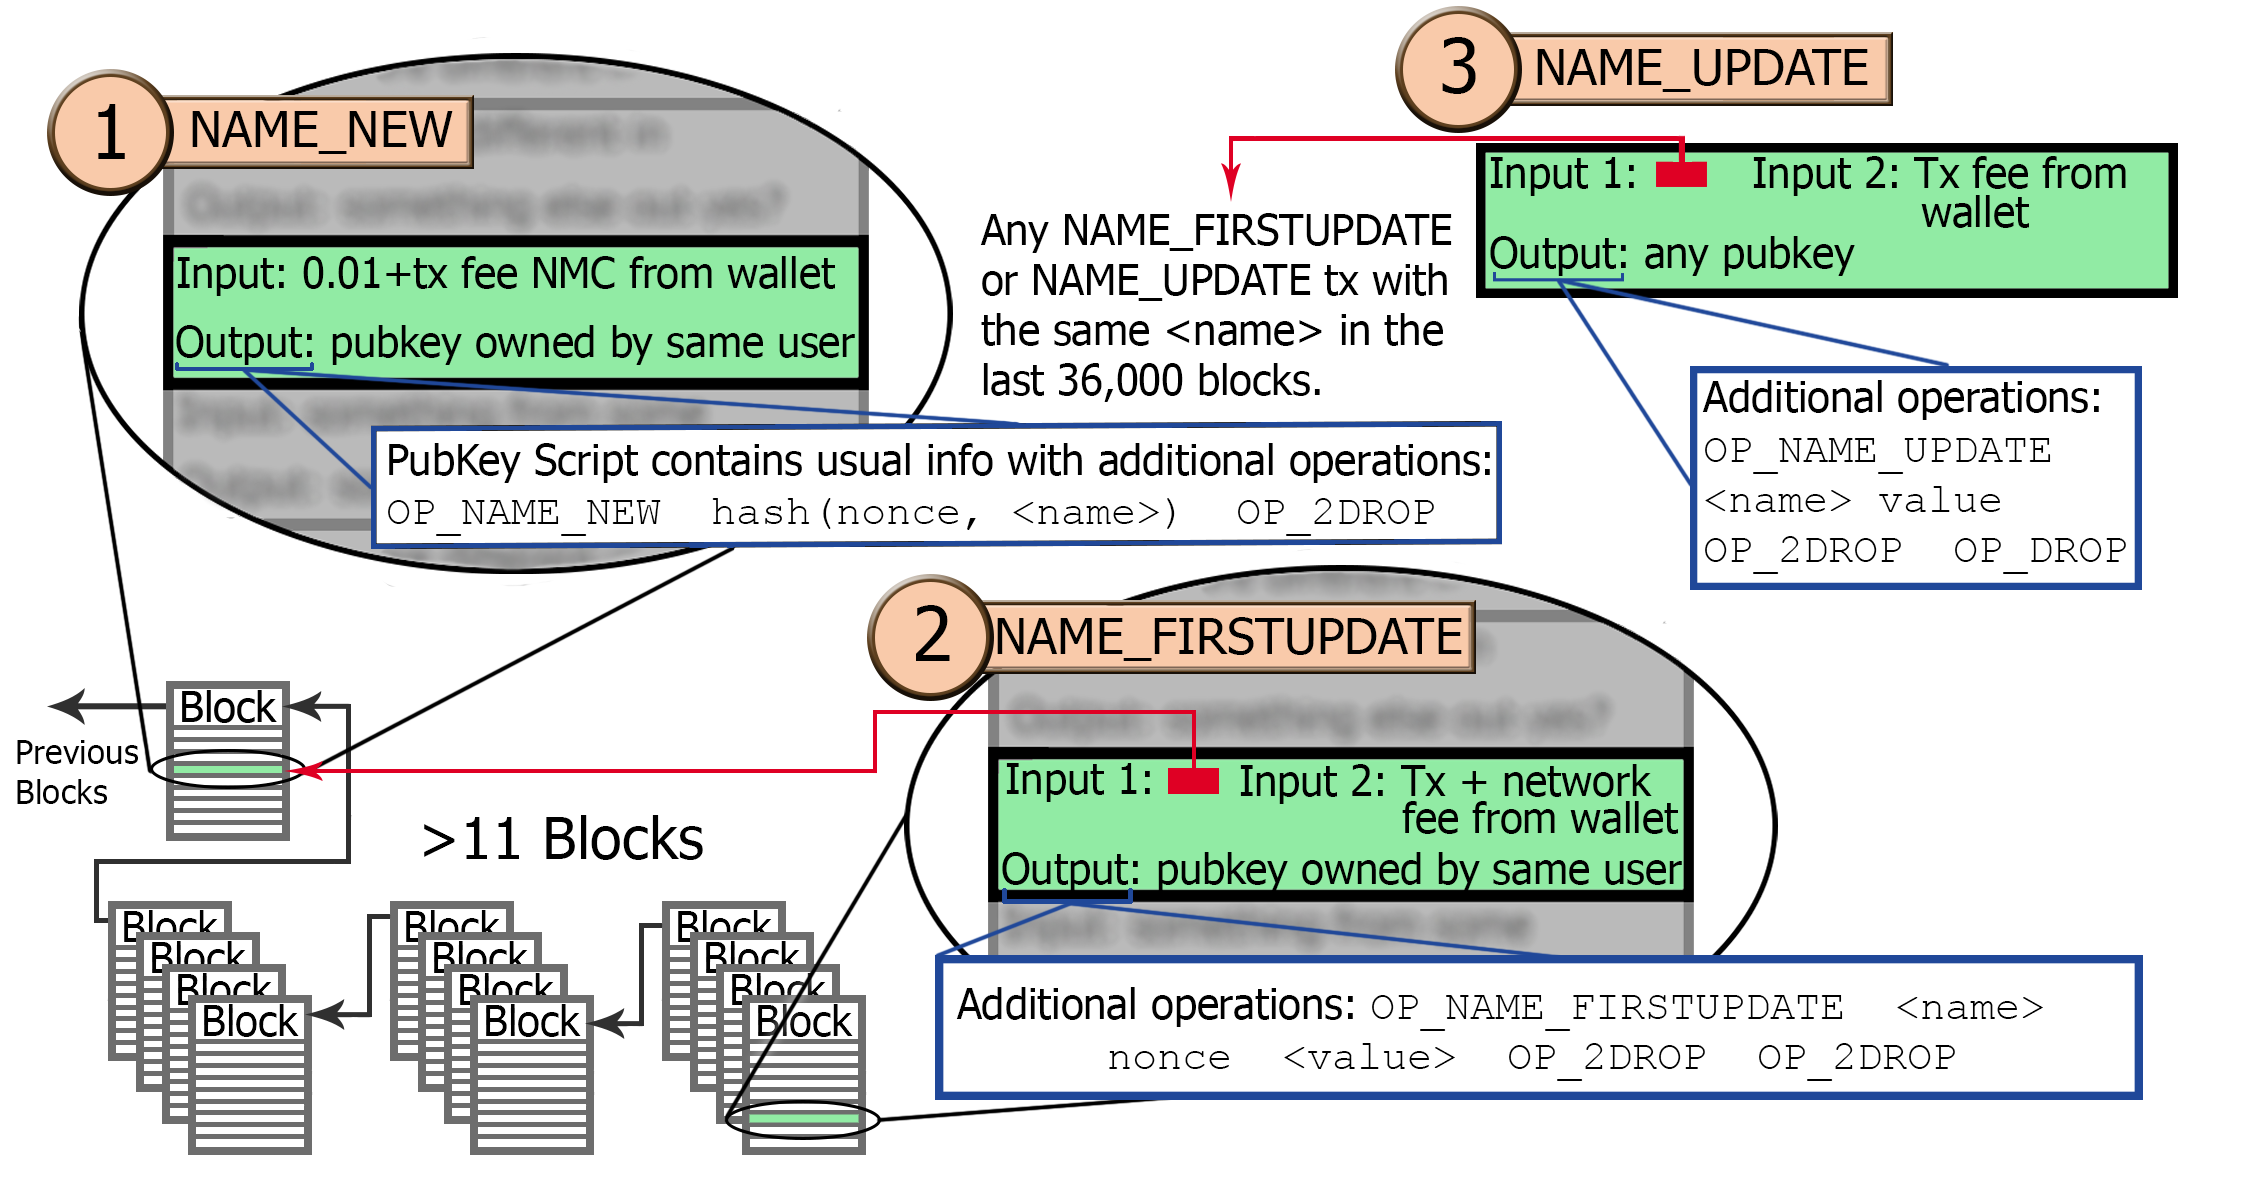
\includegraphics[width=0.95\textwidth]{registration.png}
  \caption{Namecoin Name Registration Protocol}
  \label{fig:registration}
\end{figure*}

After doing this, and waiting for 12 or more blocks on top of the one containing the NAME\_NEW transaction, the same user can use the output of the NAME\_NEW transaction as the input for the NAME\_FIRSTUPDATE transaction. Once completed, this will associate the chosen name with a value selected by the user. Similar to NAME\_NEW, NAME\_FIRSTUPDATE allows data to be posted in the block chain as part of the scriptPubKey of a special transaction. 
To create a NAME\_NEW transaction, a user will select, as input, the output of the NAME\_NEW transaction. They will then use another address they control as the output for the transaction. The scriptPubKey of this transaction will contain an NAME\_FIRSTUPDATE, the <name> desired, the random nonce used in the NAME\_NEW hash commitment, the first <value> for the name to take and some OP\_DROPs to clear this information from the stack so that they don't interfere with the rest of the locking script which comes after these extra components. In order for this transaction to be valid, a miner will verify that the <name> and the provided nonce do, in fact, hash to the commitment in the appropriate  NAME\_NEW transaction. The output of this transaction now contains the token representing the name/value pair, and whoever can unlock and spend the output can utilize the final new operation, NAME\_UPDATE.

The third and final new operation in Namecoin is the NAME\_UPDATE operation. Again, this operation arguments (the <name> and <newValue>) to be stored in the scriptPubKey of a special transaction. This transaction must have as input a NAME\_FIRSTUPDATE or NAME\_UPDATE output with the same <name>. This operation has three primary uses: updating, renewing and trading a name. If the user wants to change the value associated with a given name, they will update the name with this operation, providing a new value. If names can expire, as they do in Namecoin, then this operation can also be used to renew a name by providing a new value that is the same as the old value. In either of these cases, the user will use an address they control as an output of the transaction. The final reason to make a NAME\_UPDATE transaction is to trade the special coin to another user. In this case, the user will put, as an output, one of the other user's addresses instead of their own. Once the transaction resolves, the other user will have control over the special coin and can change the value to whatever they deem fit. Because the ownership of a <name> is associated with the ownership of the special coin, if the buyer is paying for the name with Namecoins,  the exchange between the payment and the <name> can be atomic (meaning they happen in the same transaction and either are only valid if the other is as well). 

\subsection{Mechanism Design}

In this subsection we continue discussion about the details of Namecoin. As opposed to the last section, however, this section focuses on the specifics of the mechanism design in Namecoin. 

{\bf Fees.}
Namecoin has been implemented with various fees and protocols to incentivize the behaviours of the users. The special token used in the NAME\_NEW transaction has a value of 0.01 NMC. This coin will be not be spendable like other Namecoins while it has a name attached to it, but if the name expires, then the coin will resume function as usual. For all of the transactions, NAME\_NEW, NAME\_FIRSTUPDATE, and NAME\_UPDATE, the default behaviour is to have the user tip the miner. The current expected tip, which is programmed into the Namecoin client, is 0.005 NMC on each transaction. Historically, Namecoin also had a network fee attached to the NAME\_FIRSTUPDATE transaction. The network fee is different from the transaction fee; the transaction fee is paid to the miners, whereas the network fee was destroyed (with an OP\_RETURN) when a NAME\_FIRSTUPDATE transaction was confirmed. The network fee varied over time-- it started at 50 NMC at the genesis block, but decreased by a factor of 2 every 8192 blocks (which is approximately 2 months). The purpose of the network fee was to have a large initial cost to claiming names to deter users from quickly claiming all the desirable names, but then decay off so that eventually the cost of registering a name becomes negligible. As of block 85585, the network fee became small enough that it rounds to 0 and is no longer added onto the transaction. The current implementation of Namecoin has no fees other than the transaction fee on NAME\_UPDATE transactions.

{\bf Expiration.}
Namecoin has an expiration time for names. Originally, the time period for a name to expire was 12,000 blocks, but by March 2012, the expiration period was increased to 36,000 blocks(which comes out to about 250 days). If a particular <name> hasn't been mentioned in a NAME\_FIRSTUPDATE or NAME\_UPDATE in 36,000 blocks, the name becomes available again for any user to claim with NAME\_NEW and NAME\_FIRSTUPDATE. Similarly, a NAME\_UPDATE must cite a NAME\_FIRSTUPDATE or NAME\_UPDATE that is less than 36,000 blocks old as input. 
 
\subsection{Application}

There are many different subspaces in the Namecoin namespace, and the different subspaces have different applications. When claiming a name, a user prepends the name with a subspace ID and a slash. The vision for Namecoin was to use one of these subspaces for DNS lookup in the .bit TLD. Explicitly, Namecoin names associated with .bit domains are prepended with the subspace ID {\tt d/}. If a user wanted the domain awesome.bit, they would claim the name {\tt d/awesome}, and could set the value to their server address. 

Namecoin was created so that it would be useful for any application that would benefit from an online name/value store. While {\tt d/} has the most registered names, there are also many other used subspaces in Namecoin. The most prevalent example is the online identity system OneName, which utilizes the Namecoin subspace {\tt u/}. Another example is the subspace {\tt fp/} which is used to store files in the block chain by splitting up the data in a file into many name/value pairs and having each name/value pair contain data and then point to the pair containing the next datum from the file.  Any user can create a new name subspace, which keeps the system distributed. 

